\documentclass[11pt]{article} 
\usepackage{geometry}
\geometry{letterpaper}

\usepackage{graphicx}   
\usepackage{amssymb}
\usepackage{float}
\usepackage{tabularx}
\usepackage{hyperref}
\hypersetup{
    colorlinks,
    citecolor=black,
    filecolor=black,
    linkcolor=black,
    urlcolor=black
}

\begin{document}

\begin{titlepage}
	\newcommand{\HRule}{\rule{\linewidth}{0.2mm}}
	\begin{center}
	\textsc{\LARGE McMaster University}\\[1.5cm]
	
	\textsc{\Large SmartServe}\\[0.5cm]
	\textsc{\large Software \& Mechatronics Capstone}\\[0.5cm] 

	\HRule\\[0.4cm]
		{\huge\bfseries High Level System Design}\\[0.4cm]
	\HRule\\[0.4cm]
	
	\begin{minipage}[t][][t]{0.5\textwidth}
		\begin{flushleft} \large
			\emph{Authors:}\\
			Christopher McDonald\\
			Harit Patel \\
			Janak Patel \\
			Jared Rayner  \\
			Nisarg Patel  \\
			Sam Hamel \\
			Sharon Platkin \\
		\end{flushleft}
	\end{minipage}
	~
	\begin{minipage}[t][][t]{0.4\textwidth}
		\begin{flushright} \large
			\emph{Professor:} \\
			Dr. Alan Wassyng \\[0.4cm]
			\emph{Teaching Assistants:} \\
			Bennett Mackenzie \\ 
			Nicholas Annable \\ 
			Stephen Wynn-Williams \\ 
			Viktor Smirnov
		\end{flushright}
	\end{minipage}\\[2cm]
	
	
\includegraphics[width=0.3\textwidth]{logo.png} \\
	{\large Last compiled on \today}
	\end{center}

\end{titlepage}

\tableofcontents
\listoffigures

\vfill
\begin{figure}[H]
   \centering
   \noindent\begin{tabularx}{\textwidth}{| >{\centering\arraybackslash}m{0.2\textwidth} | >{\centering\arraybackslash}m{0.2\textwidth} | >{\centering\arraybackslash}m{0.2\textwidth} | >{\centering\arraybackslash}m{0.285\textwidth} |}
   \hline 
   \textbf{Date} & \textbf{Revision} & \textbf{Comments} & \textbf{Author(s)} \\ \hline
   Dec 1, 2017 & 1.0 & Main content done for all sections & Christopher McDonald \\ \hline
   \end{tabularx}
   \caption{Revision History}
\end{figure}
\newpage
\section{Introduction}
\subsection{Project Overview}
SmartServe is an autonomous table tennis training system for table tennis players with various skill levels. SmartServe aids in diagnosing and improving a player's performance over time. The system trains table tennis players by shooting table tennis balls towards the player and detects successful returns from the player. The system can further adapt to the player's weaknesses and help them overcome it through further training. Importantly, SmartServe alleviates the problems of finding and working with a coach for players, as well as coaches trying to train multiple players simultaneously. The system will be deemed a success if the table tennis players and coaches, can enjoy and see a value added by using SmartServe.\\\\
The project started at the beginning of the Fall 2017 academic term and will conclude at the end of the Winter 2018 term. In addition, the core project team consists of final year Software and Mechatronics Engineering students who are enrolled in the MECHTRON 4TB6/SFWRENG 4G06 capstone project course.
\subsection{Document Overview}
This document will cover the entire system from a high level point of view. This means the system will be decomposed into subsystems which each have their own responsibilities and design. The subsystems will have their intended input, expected output and description of how the module will be used. In further documentation, each will be designed in a way which is abstracted from this document's perspective. The expected use cases will also be detailed to understand the expectations of the user and how each subsystem interacts with another. A more detailed view of this including timing as a factor will be detailed in the Sequence Diagram section. \\ \\
For each subsystem, its purpose will be defined with respect to the overall system. After doing so, detailed input and output parameters will be defined. The means of communication will also need to be described as these could be simple method calls to requests over some transport protocol like HTTP or TCP. The general architecture will be decided for each subsystem will be given as each needs to satisfy unique requirements and thus needs to be decided at a system level. \\ \\
To finish the document, each subsystem will be responsible for implementing some set of requirements. These requirements are outlined in the requirements document found here. % TODO link
In the ideal scenario, one subsystem will be the only one that is responsible for any one requirement but may not be the case for all the requirements. 
\subsection{Naming Conventions and Terminology}
\label{sec:definitions}
The following terms and definitions will be used throughout this document:
\begin{itemize}
\item \textbf{System}: encompasses both the hardware and software parts of SmartServe
\item \textbf{Shooting Mechanism}: refers to the part of the system that shoots the table tennis balls towards the user side (player)
\item \textbf{Team}: all team members of the core capstone project, as noted in the list of Authors
\item \textbf{User Side}: the side of the table where the user (player) is standing
\item \textbf{System Side}: the side of the table where the electromechanical system is placed; it is the opposite side of the User Side
\item \textbf{ACID}: a database transaction which is atomic, consistent, isolated and durable
\item \textbf{FPS}: frames per second
\item \textbf{GUI}: graphical user interface
\item \textbf{Pitch}: rotation along the y-axis; this rotation angle primarily dictates the range of the ball from the net to the edge of the table on the user side
\item \textbf{Yaw}: rotation along the z-axis; this rotation angle primarily dictates the panning functionality of the shooting mechanism from the right side to the left side of the table
\item \textbf{Roll}: rotation along the x-axis
\item \textbf{HTTP:} hypertext transfer protocol
\item \textbf{TCP:} transmission control protocol
\end{itemize}
\begin{figure}[H]
   \centering
   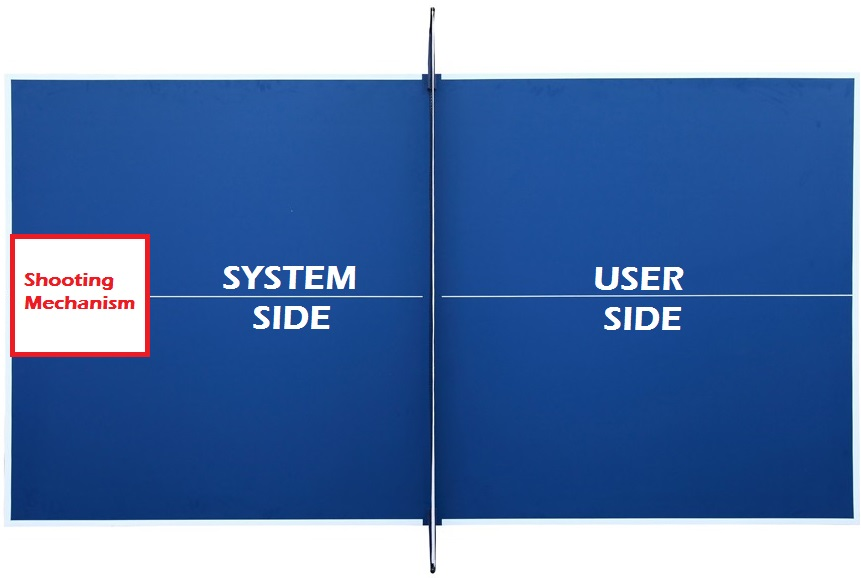
\includegraphics[width=0.75\textwidth]{img/Table-Tennis-Top-View.png} %requires the graphicx package
   \caption{Top View of the Tennis Table}
   \label{fig:table-tennis-top-view}
\end{figure}
\subsection{Project Scope}
% TODO

\section{System Description}
\subsection{System Architecture}
The system will follow a service-oriented / process-based architecture. This means that a central subsystem will interface with several services that serve a single purpose. Some subsystems will be simply told what needs to be done and others will asked for some return value. This is done to implement separation of concerns where one subsystem doesn't know everything about the system and only what is necessary to satisfy their requirements. It also allows for easy increments of versioning, where one subsystem can be used as long as it is functional and easily swapped out for a newer version with extra features or increased performance. Moreover, this system has heavy timing constraints and an unpredictable environment so some actions must be taken in absence of a service's response. For example, the computer vision may take longer to track a ball depending on its trajectory where the system must shoot another ball in order to keep the user engaged.
\subsection{Subsystems}
The system will be broken down into the subsystems with the following purposes: general managing of subsystems, computer vision to detect returns, shot recommendation, model the shot's trajectory, optimize the distance travelled by the shooting mechanism, store the data, take input and output from the user and shooting the ball toward the user. The diagram for this breakdown can be found in Figure \ref{fig:sub}.
\begin{figure}[htbp]
   \centering
   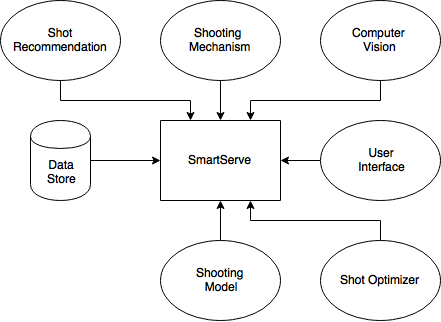
\includegraphics[width=0.6\textwidth]{img/Subsystem.png} % requires the graphicx package
   \caption{Subsystem Breakdown}
   \label{fig:sub}
\end{figure}
\subsection{Use Cases}
The diagram including all use cases can be found in Figure \ref{fig:usecase}. The user-instantiated ones will be described in detail below.
\begin{figure}[htbp]
   \centering
   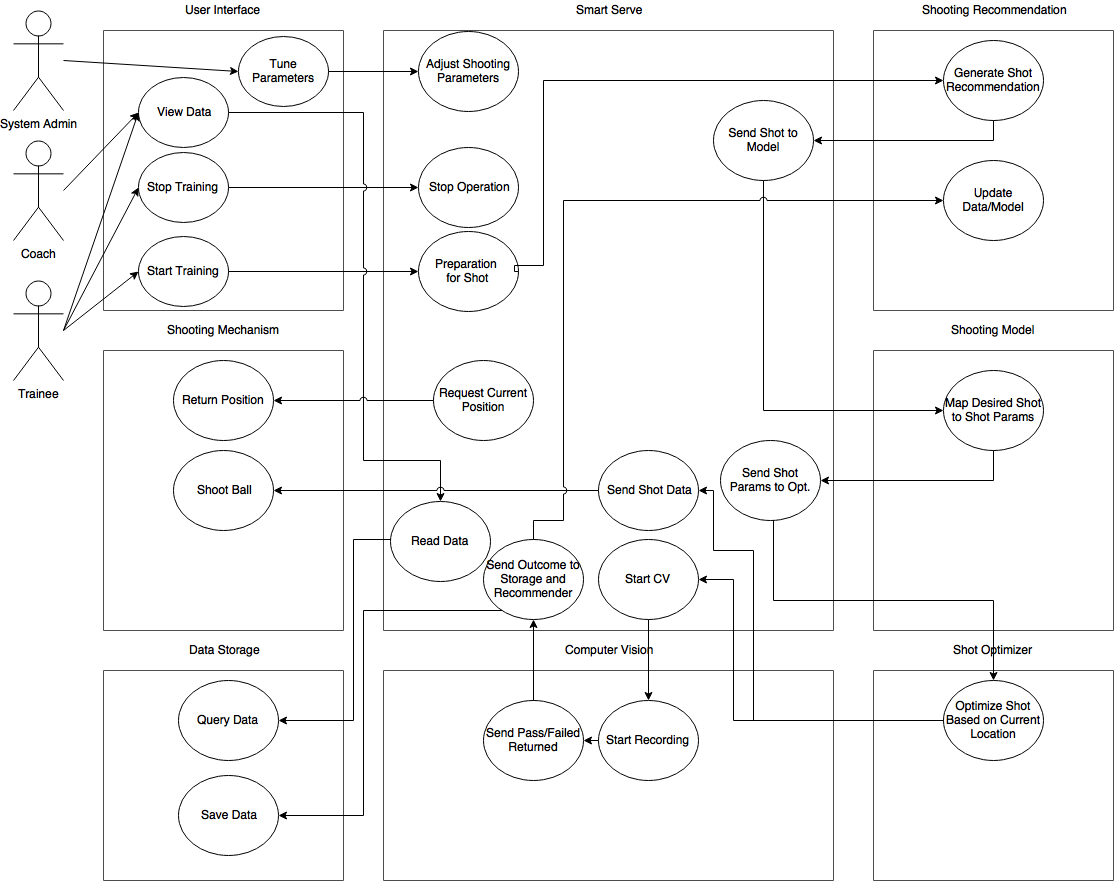
\includegraphics[width=\textwidth]{img/UseCase.png} % requires the graphicx package
   \caption{Use Case Diagram}
   \label{fig:usecase}
\end{figure}
\subsubsection*{Start Training}
\subsubsection*{Stop Training}
\subsubsection*{View Results}
\subsubsection{Use Case Diagram}
use boxes for all subsystems and list use cases
\subsection{Sequence Diagram}
basically the above with timing and loop
\subsection{Behaviour Description}
\subsubsection{Normal Operation}
\subsubsection{Error Handling}
\section{Subsystems Overview}
\subsection{SmartServe}
\subsubsection*{Purpose}
This will serve the purpose of managing the state of the system and general input and output of all other subsystems. 
\subsubsection*{Architecture}
\subsubsection*{Interface}

\subsection{Computer Vision}
\subsubsection*{Purpose}
\subsubsection*{Architecture}
\subsubsection*{Interface}

\subsection{Shot Recommendation}
\subsubsection*{Purpose}
\subsubsection*{Architecture}
\subsubsection*{Interface}

\subsection{Shooting Model}
\subsubsection*{Purpose}
\subsubsection*{Architecture}
\subsubsection*{Interface}

\subsection{Shot Optimizer}
\subsubsection*{Purpose}
\subsubsection*{Architecture}
\subsubsection*{Interface}

\subsection{Data Storage}
\subsubsection*{Purpose}
\subsubsection*{Architecture}
\subsubsection*{Interface}

\subsection{User Interface}
\subsubsection*{Purpose}
\subsubsection*{Architecture}
\subsubsection*{Interface}

\subsection{Shooting Mechanism}
\subsubsection*{Purpose}
\subsubsection*{Architecture}
\subsubsection*{Interface}
s
\section{Class Responsibility Collaboration (CRC) Cards}
who handles what requirements and who do they work with to do that
\subsection{SmartServe CRC Cards}
\subsection{Computer Vision CRC Cards CRC Cards}
\subsection{Shot Recommendation CRC Cards}
\subsection{Shooting Model CRC Cards}
\subsection{Shot Optimizer CRC Cards}
\subsection{Data Storage CRC Cards}
\subsection{User Interface CRC Cards}
\subsection{Shooting Mechanism CRC Cards}

\end{document}